\begin{figure*}[t]
\centering
% src: fig/supp_steps.pdf = python scripts/paper_supp_steps.py (CPU only; reuses the cached panels of
%   scripts/paper_cvpr_teaser.py); every printed number with its source: docs/paper/paper_supp_steps_provenance.json (printed)
% src (panels): runs/engine/pose_abc_adopt_20261113/blind, half-set 1; K = 48,000 = kb/h1/fit0/B_4536_model.pt (with the C6 copies)
% src (run 1 ruler): runs/engine/pose_abc_adopt_20261113/blind/{lean/timing.json, run_abc.log, report.json};
%   4.27 h = report.json wall_min 256.2
% src (run 2 ruler): runs/engine/abc_4090_20261117/{run_abc-4090.log, full_logs/lean/timing.json, full_logs/report.json,
%   scores/*/results.json, full_logs/lean/score_*/results.json}; 4.39 h = full_logs/report.json wall_min 263.2;
%   3 launches, 13 min redone, 16 min interruption = run_abc-4090.log "pipeline DONE" line
% src: RELION-5 24.1 h and 3.28 A = runs/engine/pose_abc_adopt_20261113/blind/comparison.json (RELION job078)
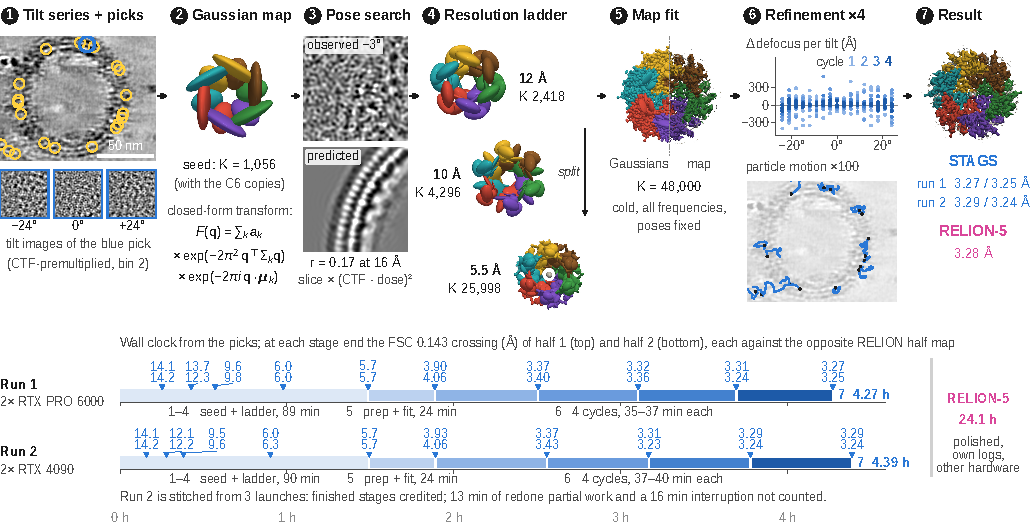
\includegraphics[width=\textwidth]{fig/supp_steps.pdf}
\caption{\textbf{STAGS step by step on EMPIAR-10164} (panels: run~1, half-set~1, central hexamer from the top).
(1)~Input: the initial picks (drawn on a denoised tomogram slice, display only) and the CTF-premultiplied tilt images of one pick.
(2)~A seed set of anisotropic 3D Gaussians, whose Fourier transform is closed-form.
(3)~Pose search: each tilt image is compared with the model's central slice times (CTF$\,\cdot\,$exposure filter)$^2$; $r$ is their correlation at the shown tilt (median over tilts).
(4)~Resolution ladder: pose search and map fit alternate from 16 to 5.5\,\AA, splitting Gaussians as resolution increases.
(5)~Cold map fit of 48,000 Gaussians at all frequencies with fixed poses (left: Gaussians, right: map).
(6)~Four refinement cycles: local pose search, per-tilt defocus and astigmatism scan (defocus changes of all half-1 tilt images), re-extraction, per-tilt geometry and per-particle motion (tracks magnified $100\times$), warm map refit.
(7)~Final map.
Rulers: wall clock from the picks for two complete blind runs of the same recipe, on a 2$\times$ RTX PRO 6000 and a 2$\times$ RTX 4090 workstation. Triangles mark stage ends and carry the FSC~0.143 crossing of each STAGS half map against the opposite RELION half map (top: half-set~1, bottom: half-set~2; reporting only, never used by the runs).
Run~2 is stitched from three launches: finished stages are credited; redone partial work and the interruption are not counted.
RELION-5 (polished) time is from its own logs on other hardware.}
\label{fig:suppl:steps}
\end{figure*}
